\subsection{ Feasibility study }
\begin{itemize}
\item Technical Feasibility As this whole project is based on C++ programming language
and Flex and Bison parsing tools, technical feasibility of this project revolves around the
technical boundaries and limitations of the C++ and these tools i.e. Flex and Bison. But as Flex and Bison is much
powerful parsing tool and C++ is powerful programming language, so
these languages are perfect to design the software under this project.\\\\
\item Economic Feasibility Almost all the softwares used in this project are Open source
and the software released under this project are Open source too and are released
under GNU GPLv3 (General Public Licence). So this project is fully economic
feasible.
\item Operational Feasibility This project is also operational feasible as it automates the
work of converting one file format into another which not only saves time. It also converts one operating system files into another. In our Project Flex and Bison tools convert Felt software files i.e. Linux based into Staad-Pro software i.e. window based. It makes conversion easily and save time.
\end{itemize}

\subsection{Software requirement specification document}
\subsection{Function Requirement}
A functional requirement defines the functions of a software system. In this software there
are tools Flex and Bison are used to develop the software. Flex and Bison tools to develop software.

\subsection{Non Functional Requirements}
The fast lexical analyser. It is the modern replacement for the classic Lex, which was developed by the Bell Laboratories in the 1970s.
Flex was originally written by Jef Poskanzer; Vern Paxson and Van Jacobson have considerably improved it. Flex is a tool for generating scanners. A scanner, sometimes called a tokenizer, is a program which recognizes lexical patterns in text. The flex program reads user-specified input files, for a description of a scanner to generate. The description is in the form of pairs of regular expressions and C code, called rules. Flex generates a C source file named, "lex.yy.c", which defines the function yylex(). The file "lex.yy.c" can be compiled and linked to produce an executable. When the executable is run, it analyzes its input for occurrences of text matching the regular expressions for each rule. Whenever it finds a match, it executes the corresponding C code.Flex and Bison files have three sections:\\
\begin{itemize}
\item The first is sort of "control" information
\item The second is the actual token/grammar definitions
\item The last is C/C++ code to be copied verbatim to the output
\end{itemize}




\subsection{Software and Hardware Requirement}
\subsection{Software requirements}
\begin{itemize}
\item Operating System: Linux/Windows
\item Tools: Flex, Bison, DXF file format
\item Programming Language: C, C++
\end{itemize}


\subsection{Hardware Requirements}
Hardware requirement of this project is any Desktop or Laptop machine for local use or a Server with minimum available configuration to make Project globally available. Hardware specifications of the machine used depends upon the hardware requirements of the Operating System installed on it. As such there are no special hardware requirements of this project.\\


\subsection{ Validation} 
For every software and techonogy, validations are must. In our parser, This software in command line based. So,there is no any database used. But we use files and validations on these files are:
\begin{itemize} 
\item When we execute files and generate output. If we gives wrong input and output file names. It show error message which is required validation for our software. 
\item Flex tool is the scanner tool which divides input into small parts called tokens. In Flex, regular expression are used as input. These tokens or regex are valid for output file. If regex are not correct, it shows message error.
\item Bison or yacc is a tool used for parsing, In this tool BNF grammar is used. Grammar is the main part of the parser. If we didn't write correct grammar. Their was problem in conversion of files.
\item In DXF converter, we use two different libraries. The use of libraries is for specific task. If libraries are not included then task does not takes place.
\end{itemize} 

\subsection{Expected hurdles}

\subsection{Regular Expression}
A regular expression processor translates a regular expression into a nondeterministic finite automaton (NFA), which is then made deterministic and run on the target text string to recognize substrings that match the regular expression. Regular expressions are so useful in computing that the various systems to specify regular expressions have evolved to provide both a basic and extended standard for the grammar and syntax; modern regular expressions heavily augment the standard. Regular expression processors are found in several search engines, search and replace dialogs of several word processors and text editors, and in the command lines of text processing utilities, such as sed and AWK.\\\\
\begin{figure} [h!]
\centering
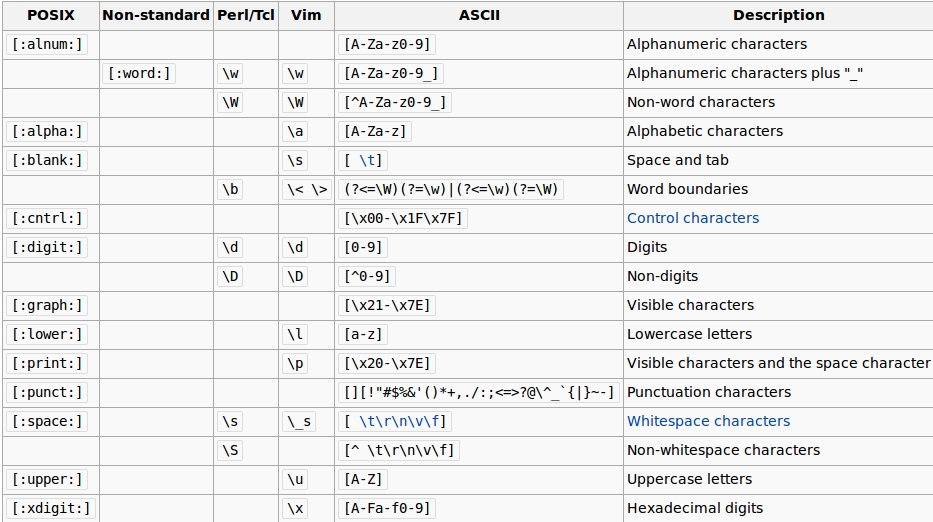
\includegraphics[scale=0.3]{images/regx.png}
\caption{meta classes}
\end{figure}

\subsection{\LaTeX{}}
\LaTeX{} is most widely used by mathematicians, scientists, 
engineers, philosophers, linguists, economists and other scholars in 
academia. As a primary or intermediate format, e.g., translating DocBook 
and other XML-based formats to PDF, \LaTeX{} is used because of the 
high quality of typesetting achievable by \TeX. The typesetting system 
offers programmable desktop publishing features and extensive facilities 
for automating most aspects of typesetting and desktop publishing, 
including numbering and cross-referencing, tables and figures, 
page layout and bibliographies.\\
\LaTeX{} is intended to provide a high-level language that
accesses the power of \TeX. \LaTeX{} essentially comprises a
collection of \TeX{} macros and a program to process \LaTeX documents. 
Because the \TeX{} formatting commands are very low-level, it is usually 
much simpler for end-users to use \LaTeX{}.

\subsection{Github}
The Git feature that really makes it stand apart from nearly every other Source Code
Management (SCM) out there is its branching model.Git allows and encourages you to
have multiple local branches that can be entirely independent of each other.The creation,
merging, and deletion of those lines of development takes seconds.\\\\

\subsection{BNF Grammer}
In computer science, BNF (Backus Normal Form or Backus–Naur Form) is one of the two main notation techniques for context-free grammars, often used to describe the syntax of languages used in computing, such as computer programming languages, document formats, instruction sets and communication protocols; the other main technique for writing context-free grammars is the van Wijngaarden form. They are applied wherever exact descriptions of languages are needed: for instance, in official language specifications, in manuals, and in textbooks on programming language theory.\\\\
In order to write a parser, we need some way to describe the rules the parser uses to
turn a sequence of tokens into a parse tree. The most common kind of language that
computer parsers handle is a context-free grammar (CFG). The standard form to write
down a CFG is Backus-Naur Form (BNF), created around 1960 to describe Algol 60
and named after two members of the Algol 60 committee. In flt-std Parser we have used BNF grammer.\\
Each line is a rule that says how to create a branch of the parse tree. In BNF, ::= can
be read “is a” or “becomes,” and | is “or,” another way to create a branch of the same
kind. The name on the left side of a rule is a symbol or term. By convention, all tokens
are considered to be symbols, but there are also symbols that are not tokens.\\
Useful BNF is invariably quite recursive, with rules that refer to themselves directly or
indirectly. These simple rules can match an arbitrarily complex sequence of additions
and multiplications by applying them recursively.\\\\
\begin{figure} [h!]
\centering
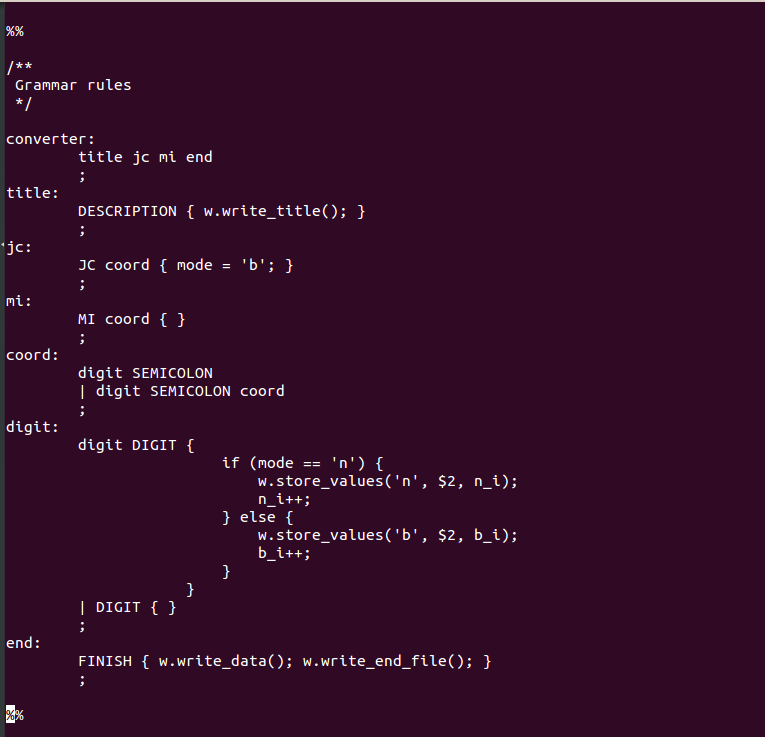
\includegraphics[scale=0.3]{images/BNF.png}
\caption{BNF Grammer in my project}
\end{figure}

\subsection{File format specifications}
A Drawing Interchange File is simply an ASCII text file with a file type of .dxf and specially formatted text. The overall organization of a DXF file is as follows:\\\\
\begin{enumerate}
\item HEADER section–General information about the drawing is found in this section of the DXF file. Each parameter has a variable name and an associated value.
\item TABLES section–This section contains definitions of named items.
\end{enumerate}

\begin{itemize}
\item Linetype table (LTYPE)
\item Layer table (LAYER)
\item Text Style table (STYLE)
\item View table (VIEW)
\item User Coordinate System table (UCS)
\item Viewport configuration table (VPORT)
\item Dimension Style table (DIMSTYLE)
\item Application Identification table (APPID)
\item BLOCKS section–This section contains Block Definition entities describing the entities that make up each Block in the drawing.
\item ENTITIES section–This section contains the drawing entities, including any Block References.
\item END OF FILE
\end{itemize}

\subsection{SDLC model to be used}  
The spiral model has four phases. A software project repeatedly passes through these
phases in iterations called Spirals.\\
\begin{itemize}
\item {\textbf{Identification}}\\
This phase starts with gathering the business requirements in the baseline spiral.
In the subsequent spirals as the product matures, identification of system require-
ments, subsystem requirements and unit requirements are all done in this phase.
This also includes understanding the system requirements by continuous communi-
cation between the customer and the system analyst. At the end of the spiral the
product is deployed in the identified market.
\item {\textbf {Design}}\\
Design phase starts with the conceptual design in the baseline spiral and involves
architectural design, logical design of modules, physical product design and final
design in the subsequent spirals.
\item {\textbf {Construct or Build}}\\
Construct phase refers to production of the actual software product at every spiral.
In the baseline spiral when the product is just thought of and the design is being
developed a POC (Proof of Concept) is developed in this phase to get customer
feedback. Then in the subsequent spirals with higher clarity on requirements and design details
a working model of the software called build is produced with a version number.
These builds are sent to customer for feedback.
\item {\textbf {Evaluation and Risk Analysis}}\\
Risk Analysis includes identifying, estimating, and monitoring technical feasibility
and management risks, such as schedule slippage and cost overrun. After testing the
build, at the end of first iteration, the customer evaluates the software and provides
feedback.


